\section{Kinect Hardware}
Microsoft brachte im November 2010 mit dem Produkt Xbox Kinect eine neues Produkt auf den Markt. Mit diesem war es möglich, ihr eigenes Produkt Xbox 360 über eine 3D-Kamera zu steuern und Spiele zu spielen. 
Mit diesem Produkt konnte erstmals ein preiswerter Sensor verwendet werden, um 3D-Bilddaten auszuwerten.
Im Folgenden wird auf die Hardware des Sensors näher eingegangen:

\begin{figure}[H]						
	\centering							
	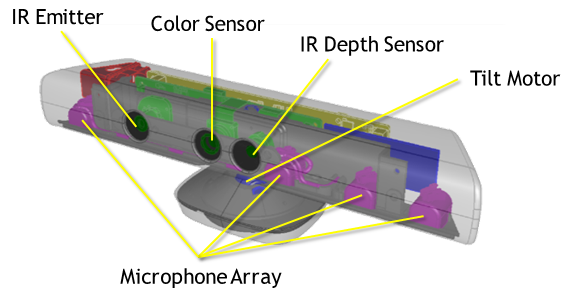
\includegraphics[scale=0.9]{Bilder/kinect_sensor_aufbau.png}			
	\caption{Aufbau Kinect\cite{ws:microsoft_kinect}}						
	\label{f:kinect_hardware}						
\end{figure}


Das Kinectmodul besteht technisch gesehen aus mehreren Komponenten, die es ermöglichen, die
im folgenden erläuterten abstrahierten Funktionen (Skelettverfolgung, Winkelextraktion, RGB-Bild)
zu realisieren. \cite{webb2012beginning}

\subsection{RGB-Kamera}

	Ein Teil der Kinect ist die RGB Kamera, die maximal eine Auflösung von 1280 x 960 Pixeln 	
	unterstützt. 
	
	Auflösung
	30 FPS bei 640x480
	12 FPS bei 1280x960
	
	Sichtfeld:
	43 Grad vertikal
	57 Grad horizontal	

\subsection{Tiefenerkennung}
	Infrarot Projektor
	CMOS Chip: depth camera 	= max resolution of 640 x 480.
	
	\todo{Triangulation}	
	\todo{PrimeSense}
	\todo{Bild Triangulation}
	
\subsection{Motor}
	Kippbarer Kopf
	
	
\subsection{Microphon Array}
	4 Mikrofone -> Für dieses Projekt irrelevant 
	(evtl. Sprachkommandos? Kinect Lib unterstützt Grammatik!!)
	Richtung d. Geräusch
	
\cite{jana2012kinect}



Rauminformationen für Software
Vorteil: Günstig, leicht zu entwickeln, da SDK vorhanden